\section{Introduction}\label{sec:taxonomy.introduction}
Chest X-ray (CXR) is a prevalent radiological examination for diagnosing lung and heart disorders, constituting a significant share of ordered imaging studies. Fast and accurate detection of different thoracic diseases, such as pneumothorax, is crucial for optimal patient care~\cite{bellaviti_Increased_2016}. However, interpreting CXRs can be challenging due to similarities between different thoracic diseases, which may result in misinterpretation even by experienced radiologists~\cite{delrue_Difficulties_2011}. Consequently, devising an accurate system to identify and localize common thoracic diseases can aid radiologists in minimizing diagnostic errors~\cite{crisp_Global_2014,silverstein_Most_2016}.
Progress in natural language processing (NLP) has enabled the collection of extensive annotated datasets such as ChestX-ray8~\cite{wang_ChestXRay8_2017}, PADCHEST~\cite{bustos_Padchest_2020}, and CheXpert~\cite{irvin_CheXpert_2019}, allowing researchers to develop more efficient and robust supervised learning algorithms.
Convolutional neural networks (CNNs) exhibit potential for learning intricate relationships between image objects. However, their training necessitates vast amounts of labeled data, which can be both expensive and time-consuming to acquire. Despite these challenges, deep learning techniques have become increasingly popular in medical imaging, especially in radiology, due to their ability to perform complex tasks with minimal human intervention~\cite{jaderberg_Spatial_2015}.
The timely diagnosis and effective treatment of diseases depend on the fast and accurate detection of anomalies in medical images. Deep learning techniques have made substantial progress in the medical imaging domain, exhibiting impressive success across various applications~\cite{litjens_Survey_2017a,eshghali_Machine_2023}.  Although recent advances in deep learning have facilitated the creation of CAD systems capable of classifying and localizing prevalent thoracic diseases using CXR images, most of these techniques have concentrated on specific diseases~\cite{jaiswal_Identifying_2019,lakhani_Deep_2017,pasa_Efficient_2019,ausawalaithong_Automatic_2018}, leaving ample opportunities to investigate a unified deep learning framework that can efficiently detect a broad spectrum of common thoracic diseases. Further, conventional classification methods are primarily designed for single-label predictions and struggle with multi-label classification, which requires predicting multiple labels for each input sample. In multi-label classification, common methods like the One-vs-All (OVA) approach exhibit limitations, including high computational complexity and an inability to capture intricate label relationships~\cite{tsoumakas_MultiLabel_2007}.
This paper aims to tackle the challenges of multi-label classification by introducing a hierarchical framework that incorporates the relationships between different classes to provide a more accurate classification framework. We propose one approach termed as ``loss-based'' for scenarios where ground truth is available, in which the proposed technique is applied to the loss function of a network (e.g., a classification or segmentation network such as DenseNet121~\cite{huang_Densely_2017} or U-Net~\cite{ronneberger_UNet_2015}). For scenarios where ground truth is not available, we propose an alternative approach termed as ``logit-based'', where the hierarchical framework is applied to the logit values of an existing pre-trained network. Logits are the output of the last layer of a neural network before applying the activation function. For multi-class problems with $K$ classes, the number of logits is $K$, and the value of each logit represents the model’s confidence in the $k$-th class being positive. For example, consider a binary classification problem where one needs to determine if an email is spam. In that case, the logit will be a single value representing the confidence that the email is spam. The higher the value of the logit, the more confident the model is that the email is spam.
The logit-based technique provides a transfer learning approach that improves classification accuracy without necessitating an extensive computational investment. The rest of this paper is structured as follows. Section~\ref{sec:taxonomy.relatedwork} discusses related work on multi-label classification and hierarchical loss functions; Section~\ref{sec:taxonomy.methods} describes the proposed techniques for integrating label hierarchy into multi-label classification techniques; Section~\ref{sec:taxonomy.results} presents experimental results using the chest radiograph dataset; and Section~\ref{sec:taxonomy.discussion} concludes the paper and outlines future research directions.
\section{Related Work}\label{sec:taxonomy.relatedwork}
The introduction of the ChestX-ray8 dataset and its associated model~\cite{wang_ChestXRay8_2017} marked a significant advancement in large-scale CXR classification, leading to numerous improvements in both modeling and dataset collection. These enhancements include the integration of ensemble methods~\cite{islam_Abnormality_2017}, attention mechanisms~\cite{guan_Diagnose_2018,liu_SDFN_2019}, and localization techniques~\cite{cai_Iterative_2018,guendel_MultiTask_2019,li_Thoracic_2018,yan_Weakly_2018}. Most early approaches use ``binary relevance'' (BR) learning, which reduces the multi-label classification problem to binary classification by training a binary classifier for each class~\cite{zhang_Review_2014}. However, BR-based techniques do not account for label dependence---either conditional (instance-specific label dependence) where in a given instance the presence or absence of one label may impact another, or marginal (dataset-specific label dependence) where certain labels may co-occur more frequently~\cite{dembczynski_Label_2012}.
Multi-label classification, unlike multi-class methods, classifies instances into multiple categories simultaneously. For example, a single chest radiograph image can have both edema and cardiomegaly~\cite{harvey_Standardised_2019,tsoumakas_MultiLabel_2007}. Significant research on integrating taxonomies through hierarchical classification was conducted prior to the advent of deep learning by extracting a set of binary hierarchical multi-label classification (HMLC) labels from pseudo-probability predictions~\cite{bi_BayesOptimal_2015}. Early methods used hierarchical and multi-label generalizations of traditional algorithms, such as nearest-neighbor or multi-layer perceptron~\cite{pourghassem_ContentBased_2008} and decision trees~\cite{dimitrovski_Hierarchical_2011}. With the rise of deep learning, the adaptation of convolutional neural networks (CNN) for hierarchical classification has gained increasing attention~\cite{guo_CNNRNN_2018,kowsari_HDLTex_2017,redmon_YOLO9000_2017,roy_TreeCNN_2020}. \\
%
\paragraph{Hierarchical Multi-Label Classification Technique: }
In many cases, the diagnosis or observation of a particular condition on a CXR (or other medical imaging data) is dependent on the presence or absence of the parent class~\cite{vaneeden_Relationship_2012}. For example, if a radiologist is trying to diagnose pneumonia in a patient, they may first look for evidence of lung consolidation (parent label) in the CXR\@. Consequently, it is possible to make more accurate diagnoses by taking into account the relationship between labels\@. However, many existing CXR classification methods do not consider the dependence between labels and instead treat each label independently. These algorithms are known as ``flat classification'' methods~\cite{alaydie_Exploiting_2012}. Furthermore, some labels at the lower levels of the hierarchy, specifically leaf nodes, have very few positive examples, making the flat learning model susceptible to negative class bias. To address these issues, we must create a model that considers the hierarchical nature of the CXR\@. \\
%
Hierarchical multi-label classification methods have been successfully implemented in a variety of domains, including text processing~\cite{aly_Hierarchical_2019}, visual recognition~\cite{bi_Mandatory_2014}, and genomic analysis~\cite{bi_BayesOptimal_2015}. A common technique~\cite{chen_Deep_2019} for exploiting such a hierarchy is to train a classifier on conditional data while ignoring all samples with negative parent-level labels and then reintroducing these samples to fine-tune the network across the entire dataset~\cite{chen_Deep_2019}. These approaches help the classifier focus on the relevant data during initial training, thus improving the prediction accuracy.  However, these techniques are computationally expensive, as they require training a classifier on conditional data and then fine-tuning it on a full dataset. This makes them difficult to apply to real-world problems, where the amount of data is often very large.   Another common strategy is a cascading architecture where different classifiers are trained at each level of the hierarchy. Although these techniques enable more granular data analysis (each classifier can focus on a specific level of the hierarchy), they require a substantial amount of computational resources. Other existing deep learning-based approaches often use complex combinations of CNNs and recurrent neural networks (RNNs)~\cite{guo_CNNRNN_2018,kowsari_HDLTex_2017}.
\section{Methods}\label{sec:taxonomy.methods}
In this study, we introduce a unique method that improves the accuracy and interpretability of multi-label classification, with potential applications in areas such as chest radiography. We propose two distinct strategies. The first strategy termed as ``loss-based'', requiring the availability of ground truth labels, incorporates the hierarchical relationships among different classes directly into the loss function. In contrast, the second strategy termed as ``logit-based'' utilizes these hierarchical relationships to modify the logit values before calculating the predicted probabilities for each class. These two strategies, which utilize a transfer learning approach, foster the use and fine-tuning of pre-existing models, thereby expanding their adaptability to new tasks. By improving the accuracy of classifying different pathologies, these techniques could potentially enhance disease diagnosis and treatment.
The proposed technique is adaptable to the available computational resources. When ample computational resources are available, the ``loss-based'' strategy can be utilized. Alternatively, in scenarios with limited computational resources, to avoid the need for optimization of the network from scratch, the ``logit-based'' strategy can be utilized.
One notable advantage of our proposed techniques lies in enhancing interpretability. By categorizing classes into a hierarchical structure and capitalizing on their relationships, the model not only improves classification performance but also provides insights into the relationships among predicted classes.
This additional layer of interpretability can help radiologists in understanding the reasoning behind the model's predictions, fostering trust in the model's output and facilitate its integration into clinical workflows. Furthermore, the hierarchical nature of the taxonomy allows radiologists to explore predictions at various levels of granularity, depending on the level of detail required for a specific case.
%
\subsection{Problem Formulation}\label{subsec:taxonomy.problem_formulation}

\subsubsection{Mathematical Formulation of Sigmoid Function}

In the context of neural networks, a logit refers to the raw, unscaled output of a neuron. This output is obtained at the last layer of a neural network model prior to the application of the sigmoid layer ~\cite{furnieles_Sigmoid_2022}. Logit values can range from negative to positive infinity. The term ``logit'' originally comes from logistic regression, and it is the inverse of the logistic sigmoid function. In machine learning, it's often desirable for our model to produce real numbers ranging from 0 to 1. Applying the sigmoid function to the logit ensures this, as the sigmoid function maps any real number to the interval \([0,1]\).
The equation representing the sigmoid function is:
\begin{equation}
p = \text{{sigmoid}}(x) = \frac{1}{1 + e^{-x}}
\end{equation}
When we apply this sigmoid function to the logit values produced by the neural network, the result is a predicted probability ranging from 0 to 1. This property is particularly useful in binary classification tasks, where the aim is to model the probability of a given input pertaining to a certain class.
In a binary classification scenarios, if we apply the sigmoid function to the logit value and obtain output \( p \), we interpret this as the model's estimated probability that the input belongs to the class.
Finally, the equation for the logit (also known as the log-odds) can be given as.
\begin{equation}
x = \text{{logit}}(p) = \log \left( \frac{p}{1 - p} \right)
\end{equation}
where \( p \) is the probability of a positive event. This function maps a probability \( p \) from the interval \((0,1)\) to any real number.
%
\subsubsection{Glossary of Symbols}\label{subsubsec:notations}

Let us define the following parameters:
\begin{itemize}
    \item  $\mathcal{C} = {\{c_k\}}_{k=1}^{K}  $: the set of classes (categories) in the multi-label dataset, where $c_k $ is the name of the $k $-th class.
    \item  $\mathcal{E} $: set of edges representing parent-child relationships between classes.
    \item  $\mathcal{G}=\left\{\mathcal{C},\mathcal{E}\right\} $:  Graph representing the taxonomy of thoracic diseases.
    \item  $c_j=\Lambda (c_k) \in \mathcal{C}$: parent class of class $c_k $ in graph $\mathcal{G} $.
    \item  $\mathcal{J}(c_j) \subset \mathcal{C}$: set of child classes of class $c_j$ in graph $\mathcal{G} $
    \item  $y_k^{(i)} \in \{0,1\} $: true label for the $k $-th class of instance $i $.
    \item  $q_k^{(i)} \in \left( -\infty,0 \right) $: logits obtained in the last layer of the neural network model before the sigmoid layer.
    \item  $p_k^{(i)} = \text{sigmoid}\left(q_k^{(i)}\right) = \frac{1}{1+\exp{\left(-q_k^{(i)}\right)}} $: predicted probability for the $k $-th class ($c_k) $ of instance $i $ with a value between 0 and 1. $p_k^{(i)} $ represents the likelihood that class $k $ is present in instance $i $ and is obtained by passing logits $q_k^{(i)} $ through a sigmoid function.
    \item  $\theta_k $: Binarization threshold for class $k $.  To obtain this, we can utilize any existing thresholding technique (for example, in one technique, we analyze the ROC curve and find the corresponding threshold where the difference between the true positive rate (sensitivity) and false positive rate (1-specificity) is maximum; alternatively, we could simply use $0.5 $).
    \item  $t_k^{(i)}=\left\{\begin{array}{lc}1&\text{if}\;p_k^{(i)} \geq \theta_k\\0&\text{otherwise.}\end{array}\right. $: predicted label obtained by binarizing the $p_k^{(i)} $
    \item  ${\widehat p}_k^{(i)} \in (0,1) $: updated predicted probability for the $k $-th class of instance $i $ with a value between 0 and 1.
    \item  $\widehat{t}_k^{(i)}=\left\{\begin{array}{lc}1&\text{if}\;\widehat{p}_k^{(i)}\geq\theta_k\\0&\text{otherwise.}\end{array}\right. $: updated predicted label for the $k $-th class of instance $i $.
    \item $K $: number of categories (aka classes) in a multi-class, multi-label problem. For example, suppose that we have a dataset that is labeled for the presence of cats, dogs, and rabbits in any given image. If a given image $X^{(i)} $ has cats and dogs but not rabbits, then $Y^{(i)} = \{1,1,0\} $.
    \item  $N $: Number of instances.
    \item $X^{(i)} $: Data for instance $i$.
    \item     $Y^{(i)}=\left\{y_1^{(i)},y_2^{(i)},\;\dots,y_{K}^{(i)}\right\} $: True label set for instance $i $. For example, consider a dataset that is labeled for the presence of cats, dogs, and rabbits in any given instance. If a given instance $X^{(i)} $ has cats and dogs but not rabbits, then $Y^{(i)}=\{1,1,0\} $.
    \item     $P^{(i)} = {\left\{ p_k^{(i)} \right\}}_{k=1}^{K} $: Predicted probability set obtained in the output of the classifier $F(\cdot) $ representing the probability that each class $k $ is present in the sample.
    \item  $T^{(i)} = {\left\{t_k^{(i)}\right\}}_{k=1}^{K} $: predicted label set for instance $i $.
    \item  $\mathbb{X} = {\left\{X^{(i)}\right\}}_{i=1}^{N} $: Set of all instances.
    \item  $\mathbb{Y} = {\left\{Y^{(i)}\right\}}_{i=1}^{N} $: Set of all true labels.
    \item $\mathbb{D}=\left\{\mathbb{X},\mathbb{Y}\right\} $: Dataset containing all instances and all true labels.
    % \item  $\mathbb{D}_{\text{phase1}},\mathbb{D}_{\text{phase2}} $: randomly selected subsets of the $\mathbb{D} $ dataset used for phase1: training the machine learning model and phase2: applying the proposed taxonomy technique. $\mathbb{D}_{\text{phase1}}\cup\;\mathbb{D}_{\text{phase2}}=\mathbb{D} $ and $\mathbb{D}_{\text{phase1}} \bigcap \mathbb{D}_{\text{phase2}} = \varnothing $
    \item  $l_k^{(i)} = \mathcal{L} \left(y_k^{(i)},p_k^{(i)}\right) $:  $\mathcal{L}(\cdot)$ is an arbitrary loss function (e.g., binary cross entropy) that takes the true label $y_k^{(i)}$ and predicted probability $p_k^{(i)}$ for class $k$ and instance $i$ and outputs the loss value $l_k^{(i)} $. We refer to this as the ``base loss function'' throughout this paper.
    \item  $\text{Loss}(\theta) $: Measured loss for all classes and instances. This value is obtained using a modified version of the base loss function $\mathcal{L}(\cdot) $ (e.g., with added regularization, etc.).
    \item  $\omega_k^{(i)} $: Estimated weight for $k$-th class $c_k $ of instance $i $ with respect to its parent class $\Gamma_k $.
    \item  ${\widehat l}_k^{(i)} = \omega_k^{(i)} \; l_k^{(i)} $: updated loss for class $k $ and instance $i $.
    % \item  ${\widehat p}_k^{(i)}=\omega_k^{(i)}\;p_k^{(i)} $: updated predicted probability for the $k $ -th class.
\end{itemize}
Let us define the multi-label classification problem as follows. Let $\mathbb{X} = {\left\{X^{(i)}\right\}}_{i=1}^{N} $ be a set of $N $ chest radiograph images and $\mathbb{Y} = {\left\{Y^{(i)}\right\}}_{i=1}^{N} $ be their corresponding ground truth labels. The ground-truth labels for the dataset were provided by experienced radiologists who annotated each image with the corresponding abnormalities.
Given the set of disease classes $\mathcal{C} = \{c_1,c_2,\dots,c_K\} $, let us define a  graph $\mathcal{G}=\left\{\mathcal{C},\mathcal{E}\right\} $ representing the taxonomy of thoracic diseases, where $\mathcal{E}$ is the set of edges representing parent-child relationships between these classes. For each node $c_k \in \mathcal{C} $, let $\Lambda_k$ be the parent node of class $c_k $ and let $\mathcal{J}_k\subset \mathcal{C} $ be the set of child classes of class $c_k $ in graph $\mathcal{G}$. \\
In the context of multi-label classification problems, each sample may have multiple labels assigned to it simultaneously. To this end, we use a deep neural network, with multiple hidden layers and the sigmoid activation function in the final layer. Let's denote the input to this neural network by $x^{(i)}$, which represents the instance $i$'s data (data can be of type 1D feature vector, 2D image, or 3D volume). This network is trained to predict the probabilities for each class being present in a given sample. Hence, the output of the final layer of the neural network for instance $i$ is passed through a sigmoid function to generate a set of values, each ranging from 0 to 1, corresponding to the label set $\mathcal{C} $.
The outcome of this operation is a set of $K $ predicted probabilities $P^{(i)}={\left\{p_k^{(i)}\right\}}_{k=1}^{K} $. Each of these predicted probabilities, derived from the sigmoid activation function, can be interpreted as the likelihood that the input sample belongs to each class.
Furthermore, let $\omega_k^{(i)} $ be a scalar weight assigned to the class $c_k $ of instance $i $ with respect to its parent class $\Lambda_k$.
Each of these predicted probabilities, derived from the sigmoid activation function, can be interpreted as the likelihood that the input sample belongs to each class. A loss function is utilized to quantify the similarity between predicted probabilities and true labels. This function guides the learning process of the neural network by providing a measure of the prediction error, which is minimized during the training phase.
Let us denote the loss value as $l_k = \mathcal{L} \left(p_k^{(i)},y_k^{(i)}\right),\hspace{0.33em}k \in \{1,2,\dots,K\} $ where $\mathcal{L}(\cdot) $ is an appropriate single-class loss function for the task (e.g., binary cross-entropy, Dice, etc.) that is used to calculate the difference between the predicted probability $p_k^{(i)} $ and the true class label $y_k^{(i)} $ for instance $i$ and class $k $.
\subsection{Label Taxonomy Structure}\label{subsec:label-taxonomy-and-hierarchy}
To exploit the hierarchical relationships between thoracic abnormalities, the first step is to define a disease taxonomy that demonstrates different abnormalities’ interrelationships. In this taxonomy, diseases are structured hierarchically in a graph, with higher levels representing broader disease categories and lower levels representing more nuanced distinctions between related diseases. The taxonomy is structured such that if a disease is present then its parent disease is also present. Furthermore, in presence of multiple parent classes for a given child class, the taxonomy structure only utilizes the more dominant parent (e.g., if class $c_1$ has two parent classes $c_3$ and $c_5$ , while the $c_5$ is also the parent of $c_3$ class, in this scenario, we assume $c_5$ as the parent class of both $c_1$ and $c_3$.
For example, pleural effusion and pneumothorax can be classified as subcategories of pleural abnormalities, whereas atelectasis and consolidation can be classified under pulmonary opacity. This hierarchical structure enables the model to take advantage of the relationships between diseases to improve its classification performance.
In medical imaging, classes are frequently organized as graphs to represent the hierarchical relationships between different classes. For example, a graph can be used to represent the human body's organs, with each node representing a different organ and the edges representing the relationships between organs (e.g., the liver is part of the abdominal cavity). Using a graph structure for labels in medical imaging has a number of advantages, including improved accuracy and interpretability of classification algorithms, which are essential for making sense of the vast amounts of data generated by medical imaging technologies. In medical imaging, hierarchies of labels are typically constructed by subject matter experts with a comprehensive understanding of human anatomy and physiology, such as radiologists.
A comprehensive label taxonomy for lung diseases was developed based on the taxonomies presented by Irvin~\cite{irvin_CheXpert_2019} for the CheXpert dataset and Chen~\cite{chen_Deep_2020} for the PADCHEST~\cite{bustos_Padchest_2020} and the CXR arm of the prostate, lung, colorectal and ovarian (PLCO)~\cite{gohagan_Prostate_2000} datasets. This unified taxonomical structure (explained in Section~\ref{subsec:label-taxonomy-and-hierarchy} is designed to be applied to various chest radiography datasets. The developed taxonomy structure is depicted in Figure~\ref{fig:taxonomy.fig.1.taxonomy_structure}.
\subsection{Approach 1: Conditional Predicted Probability}\label{subsec:taxonomy.method.approach1}
When computational resources are limited, this technique can be applied to test samples without the need to fine-tune the pre-trained, multi-label classification model. This adaptability ensures that the benefits of considering hierarchical relationships between labels can be realized in a wide range of practical scenarios, without imposing excessive computational requirements.
Directly updating the predicted probabilities presents potential benefits, including the following:
\begin{itemize}
    \item  \textbf{Simplicity:} Direct modification of predicted probabilities eliminates the need for substantial changes to the loss function, thus facilitating implementation.
    \item  \textbf{Faster convergence:} In some cases, direct updates can accelerate convergence due to a more accurate representation of hierarchical relationships, thus reducing the overall training time.
    \item  \textbf{Improved performance in specific scenarios:} Depending on the problem and dataset, direct updates may provide superior performance in certain circumstances, especially when incorporating class relationships into the loss function is challenging.
    \item  \textbf{Easier calibration:} Direct modification of predicted probabilities can facilitate calibration of the model output to more closely match the true label distribution.
\end{itemize}
The proposed technique provides an easy way to improve the performance of existing pre-trained models during inference time by updating the value of the predicted logit for each class that was obtained at the last layer of the neural network based on the predicted logit of its corresponding parent class. The aim is to calculate the conditional predicted probability for each class $k $ and instance $i $, taking into account the predicted probability of the parent class. We can formalize this by defining a new predicted probability for the $k $ -th class $(c_k) $ and instance $i $ as follows.
\begin{equation}
    \widehat{p}_k^{(i)} = \frac{1}{ 1 + \exp \left(-\left(q_k^{(i)} + \alpha_{k,j} q_j^{(i)} \right)\right) }
    \label{eq:taxonomy.eq.1.pred.approach1}
\end{equation}
where $j=\Lambda_k$ is the index of the parent class of the $k$-th class, and $\alpha_{k,j} $ is the hyperparameter that controls the influence of different parent class logits on child class logits.
When $\alpha_{k,j}=0 $, there is no influence from the parent class $c_j$ on the child class $c_k$.  By carefully selecting appropriate hyperparameter values, this transfer learning-based technique can be employed to effectively adjust the predicted probabilities of each class, considering the hierarchical relationship between classes, and potentially improving classification accuracy.
\subsubsection{Parameter Selection and Tuning}
The selection of appropriate hyperparameters is crucial for the effectiveness of the proposed transfer learning-based technique. In this study, we employ a systematic approach to tune the hyperparameters $\alpha_{k,j} $, which controls the dependency between the predicted probabilities of the child and parent classes. We utilize a grid search method along with cross-validation to determine the optimal values for these hyperparameters. The search space for both hyperparameters is defined based on preliminary experiments and domain knowledge, ensuring a balance between model complexity and predictive performance.
\subsection{Approach 2: Conditional Loss}\label{subsec:taxonomy.method.approach2}
In a second approach, we propose a similar concept to the approach discussed in section~\ref{subsec:taxonomy.method.approach1}, however, rather than directly updating the predicted probability of each class, we instead update the loss value of each class based on the loss values of its parent classes. In the previous approach, we directly updated the predicted probability so that it could be applied unsupervised to existing pre-trained models. Although this method is highly useful during inference time, it presents some challenges if we use it during the optimization phase of our classifier model. Among these disadvantages are the following.
\begin{itemize}
    \item \textbf{Inconsistency with the optimization process:} Direct updating of predicted probabilities can misalign with the optimization procedure, which typically minimizes the loss function, potentially resulting in learning inconsistencies.
    \item \textbf{Difficulty in fine-tuning:} Direct updates can complicate fine-tuning the method's impact on the model, whereas adjusting the influence of various components is often simpler when updating the loss value through weighting factors or hyperparameters.
    \item \textbf{Potential overfitting:} Direct modification of predicted probabilities could inadvertently overfit the model to particular hierarchical relationships in the training data, thus hindering generalization to unseen data.
\end{itemize}
The utilization of the loss function based approach can prove advantageous in certain scenarios, particularly in the context of multi-label classification tasks that involve hierarchical relationships, as it offers numerous benefits.
\begin{itemize}
    \item \textbf{Emphasis on error minimization:}The loss values represent the difference between the predictions made by the model and the actual labels provided as ground-truth. Incorporating parent class loss values into child class loss calculations aims to minimize errors throughout the hierarchy, thereby assuring accurate predictions for both parent and child classes.
    \item \textbf{Enhanced gradient propagation:} During the training of deep learning models, the model parameters are updated by backpropagating gradients through layers. Incorporating the loss values of the parent class through the calculation of the loss for the child class improves the connections between the parent and child classes with respect to the propagation of gradients. This may lead to more effective acquisition of hierarchical associations and expedited convergence in the course of training.
    \item \textbf{Robustness to label noise:} Real-world datasets may exhibit inconsistencies or noise in their ground truth labels. The inclusion of loss values from parent classes in the computation of loss values for child classes enhances the consistency of the hierarchy by penalizing deviations from anticipated parent-child associations. This approach improves the model's resilience to possible label inaccuracies in the dataset.
    \item \textbf{Improved interpretability:} Employing loss values instead of predicted probabilities facilitates a more straightforward comprehension of the model's ability to capture hierarchical interrelationships among classes. The impact of high loss values on parent classes is more pronounced on the losses of their corresponding child classes, indicating the necessity to improve specific areas to better reflect these associations.
\end{itemize}
\subsubsection{Formulation of the Proposed Technique}
In multi-label classification problems, where each sample may belong to multiple classes, it is often necessary to combine the loss values for all classes to effectively train the model. Various methods can be employed to achieve this, depending on the specific problem. A common approach is to calculate the average loss across all classes for each sample by summing the losses for each class of a given sample and dividing the sum by the total number of classes to which the sample belongs. This method is effective when all classes are independent, of equal importance, and warrant equal weight in the total loss calculation. For example, in the case of cross-entropy loss, we have
\begin{equation}
    l_k = -\left(y_k^{(i)}\log(p_k^{(i)}) + (1 - y_k^{(i)})\log(1 - p_k^{(i)})\right)
    \label{eq:taxonomy.eq.2.loss}
\end{equation}
\begin{equation}
    \text{Loss}(\theta) = \sum_{i=1}^{N}\sum_{k=1}^{K}l_k
    \label{eq:taxonomy.eq.3.totalloss}
\end{equation}
In this formulation, the objective is to minimize the loss function with respect to the model parameters $\theta $, resulting in an optimal set of parameters that produce accurate predictions for multi-label classification tasks. However, class independence and equal importance between different classes cannot always be assumed. Inclusion of a hierarchical penalty or regularization term in the loss function is one way to push the loss function to take the taxonomy into account when optimizing the model hyperparameters (weights and biases). We use a regularization term $\beta_k$  to penalize the loss for class $c_k$ for each instance $i $ in which the probability that its parent class $c_j$ exists in that instance is low. This can be represented mathematically by adding a hierarchical penalty term $H(c_k \vert c_j)$ for the class $c_k$ with respect to its corresponding parent class $c_j$ as follows.
\begin{equation}
    \widehat{l}_{k}^{(i)} = l_{k}^{(i)}+\beta_k H \left(c_k \vert c_j \right)
    \label{eq:taxonomy.eq.3.newloss}
\end{equation}
where $c_j=\Lambda(c_k)$, and $\beta_k $ is the hyperparameter that balances the contributions of the class k's own loss value and its parent classes' loss values.
There are multiple ways to define the hierarchical penalty. For example, we can define it as the loss value of the parent class $l_j=L\left(y_j^{(i)},p_j^{(i)}\right) $ as follows.
\begin{equation}
    H(k \vert j)=\mathcal{L} \left(y_j^{(i)},p_j^{(i)}\right)
    \label{eq:taxonomy.eq.4.hierarchical_penalty1}
\end{equation}
Another approach to incorporating the interdependence between different classes into the loss function is to apply the loss function $\mathcal{L} $ to the true label of the parent class and the predicted probability of the child class as follows.
\begin{equation}
    H\left(k\vert j\right) = \mathcal{L} \left(y_j^{(i)},p_k^{(i)}\right)
    \label{eq:taxonomy.eq.5.hierarchical_penalty2}
\end{equation}
In both Equations~(\ref{eq:taxonomy.eq.4.hierarchical_penalty1}) and~(\ref{eq:taxonomy.eq.5.hierarchical_penalty2}) the penalization term encourages the model to correctly predict the corresponding parent class when predicting the child class, ensuring that the predicted label set adheres to the hierarchical structure. In the aforementioned approach, we assume a linear relationship between child and parent losses, which can simplify the optimization process. However, this may not always accurately capture the relationship between the parent-child classes, as the relationship may not always be linear. Furthermore, the impact of the parent's loss on the total loss could be less significant, particularly if the child's loss is considerably greater than the parent's loss.
To address this problem, we can modify the loss measurements presented in Equations~(\ref{eq:taxonomy.eq.4.hierarchical_penalty1}) and~(\ref{eq:taxonomy.eq.5.hierarchical_penalty2}) to be based on the multiplication of losses rather than their addition.
Multiplying losses allows for a more flexible relationship between the child and parent classes, as it can model both linear and nonlinear relationships. Furthermore, the parent's loss can have a more significant impact on the total loss, since it is multiplied by the child's loss, ensuring that the hierarchical relationships are better captured. To achieve this, we can define the new loss as follows.
\begin{equation}
    \label{eq:taxonomy.eq.7.newloss}
    \widehat{l}_k^{(i)} = l_k^{(i)} H \left( c_k \vert c_j \right)
\end{equation}
where the hierarchical penalty term is defined as follows.
\begin{equation}
    \label{eq:taxonomy.eq.8.hierarchical_penalty.loss}
    H(k \vert j) = \left\{ \begin{array}{lc}1 & \text{otherwise.} \\ a_k l_j^{(i)} + \beta_k & c_j \text{ has a parent} \end{array} \right.
\end{equation}
where $c_j $ is the parent class of the $c_k $ class, and $l_j $ is the parent loss value for instance $i $.
The modified loss function in Equation~(\ref{eq:taxonomy.eq.7.newloss}) aims to ensure that predictions adhere to hierarchical relationships between classes by penalizing deviations from these established relationships. By adjusting the parameters $\alpha_k $ and $\beta_k $, we can regulate the degree to which hierarchical information influences the learning process.
\subsection{Updating Loss Values and Predicted Probabilities}\label{subsec:updating-loss-values-and-predicted-probabilities}
In the previous section, we introduced a taxonomy-based loss function with the goal of improving the classification accuracy of multi-class problems. However, one of the main advantages of our proposed technique is that it enables efficient utilization of pre-trained models and leverages the existing knowledge, thus reducing the computational cost and training time associated with re-optimization. In this section, we illustrate how both of our proposed approaches can be seamlessly integrated into the existing classification framework without the necessity to re-run the optimization phase of our classifier (e.g., DenseNet121). This can be achieved by focusing on updating the loss values (approach 2 shown in section~\ref{subsec:taxonomy.method.approach2}) and predicted probabilities (approach 1 shown in section~\ref{subsec:taxonomy.method.approach1}) to incorporate the hierarchical relationships present in the taxonomy structure.
During a training phase of a classifier (e.g., DenseNet121), an optimization algorithm such as gradient descent is used to determine the predicted probabilities that minimize the loss across the entire dataset. However, this approach is only valid during the training phase and only shows the predicted probability with respect to the original loss values measured by the classifier.
In the following, we show how to calculate the updated predicted probabilities from their updated loss values obtained from Equation~(\ref{eq:taxonomy.eq.7.newloss}) without re-doing the optimization process. Let us assume that binary cross entropy is used for the choice of the loss function $\mathcal{L}(\cdot) $. Let us denote $\widehat{q}_k^{(i)} , \widehat{p}_k^{(i)} $ as the updated values for logit and predicted probability of class $k $ and instance $i $ after applying the proposed technique. As previously discussed, to calculate the predicted probabilities, we need to pass the logits ${\widehat q}_k^{(i)} $ into a sigmoid function as shown below:
\begin{equation}
    \label{eq:taxonomy.eq.9.sigmoid}
    \widehat{p}_k^{(i)}=\text{sigmoid}\left(\widehat{q}_k^{(i)}\right)=\frac1{1+\exp\left(-\widehat{q}_k^{(i)}\right)}
\end{equation}
The sigmoid activation function maps any value to a number between zero and one. The gradient of the sigmoid function (shown below) provides the direction in which the predicted probability must be updated.
\begin{equation}
    \label{eq:taxonomy.eq.10.sigmoidprime}
    \text{sigmoid}'\left(\widehat{q}_k^{(i)}\right)=\frac{\partial{\text{sigmoid}}}{\partial{q}}=\text{sigmoid}\left(\widehat{q}_k^{(i)}\right)\left(1-\text{sigmoid}\left(\widehat{q}_k^{(i)}\right)\right)=\widehat{p}_k^{(i)}\left(1-\widehat{p}_k^{(i)}\right)
\end{equation}
The loss gradient gives us the direction in which the predicted probability needs to be updated to minimize the loss. The gradient of the binary cross-entropy loss is calculated as follows:
\begin{equation}
    \label{eq:taxonomy.eq.11.lossgradient}
    \frac{\partial \mathcal{L} \left( \widehat{p}_k^{(i)},\;y_k^{(i)}\right)}{\partial \widehat{p}}=\frac{y_k^{(i)}}{\widehat{p}_k^{(i)}}-\frac{1-y_k^{(i)}}{1-\widehat{p}_k^{(i)}}
\end{equation}
where $y_k^{(i)}\; $and ${\widehat p}_k^{(i)}\; $ are the true label and predicted probability, respectively, for instance $i $ and class $k $.
In the following equations, we show how we can use the predicted probability, the gradient loss shown in Equation~(\ref{eq:taxonomy.eq.11.lossgradient}) and the derivative of the sigmoid function shown in Equation~(\ref{eq:taxonomy.eq.10.sigmoidprime}) to calculate the updated predicted probability.
\begin{equation}
\label{eq:taxonomy.eq.12.newpredelement}
\frac{\partial \mathcal{L}\left(p_k^{(i)},\; y_k^{(i)}\right)}{\partial p}\;\text{sigmoid}^{'}\left(\widehat{q}_k^{(i)}\right)=\left(\frac{y_k^{(i)}}{\widehat{p}_k^{(i)}}-\frac{1-y_k^{(i)}}{1-\widehat{p}_k^{(i)}}\right)\widehat{p}_k^{(i)}\left(1-\widehat{p}_k^{(i)}\right)=y_k^{(i)}-\widehat{p}_k^{(i)}
\end{equation}
Hence, we can conclude the following.
\begin{equation}
    \label{eq:taxonomy.eq.13.newpred}
    \begin{array}{@{}l}\hat{p}_{k}^{(i)} = \left\{\begin{array}{lc}-\frac{\partial \mathcal{L}\left(p_k^{(i)},\;y_k^{(i)}\right)}{\partial p}\;\text{sigmoid}^{'}\left(\widehat{q}_k^{(i)}\right)\text{+1} & y=1\\-\frac{\partial \mathcal{L}\left(p_k^{(i)},\;y_k^{(i)}\right)}{\partial p}\;\text{sigmoid}^{'}\left(\widehat{q}_k^{(i)}\right) & \text{otherwise.} \end{array}\right.\end{array}
\end{equation}
We would like to modify this equation so that it does not directly depend on the true value and instead rely on the gradient loss. If we simplify the loss gradient shown in Equation~(\ref{eq:taxonomy.eq.11.lossgradient})  we obtain the following:
\begin{equation}
    \label{eq:taxonomy.eq.14.newlossgradient}
    \frac{\partial \mathcal{L}(\widehat{p}_k^{(i)}, y_k^{(i)})}{\partial \widehat{p}} = \frac{y_k^{(i)}}{\widehat{p}_k^{(i)}} - \frac{1 - y_k^{(i)}}{1 - \widehat{p}_k^{(i)}} = \frac{y_k^{(i)} - \widehat{p}_k^{(i)}}{\widehat{p}_k^{(i)}(1 - \widehat{p}_k^{(i)})}
\end{equation}
In this equation, we can see that when the true label is positive $\left(y_k^{(i)}=1\right) $, the loss gradient can only be 0 or a positive number. Similarly, when $\left(y_k^{(i)}=0\right) $, the loss gradient can only take the value 0 or a negative number. Thus, we can modify the Equation~(\ref{eq:taxonomy.eq.13.newpred})  to look as follows.
\begin{equation}
    \label{eq:taxonomy.eq.15.newpred}
    \widehat{p}_k^{(i)} =
    \begin{cases}
        -\frac{\partial \mathcal{L}(\widehat{p}_k^{(i)}, y_k^{(i)})}{\partial \widehat{p}} \, \text{sigmoid}^{\prime}(q_k^{(i)}) + 1 & \text{if} \quad \frac{\partial \mathcal{L}(\widehat{p}_k^{(i)}, y_k^{(i)})}{\partial \widehat{p}} \geq 0 \\
        -\frac{\partial \mathcal{L}(\widehat{p}_k^{(i)}, y_k^{(i)})}{\partial \widehat{p}} \, \text{sigmoid}^{\prime}(q_k^{(i)}) & \text{otherwise.}
    \end{cases}
\end{equation}
Finally, the Equation~(\ref{eq:taxonomy.eq.15.newpred}) can be simplified as follows.
\begin{equation}
    \label{eq:taxonomy.eq.16.newpred}
    \widehat{p}_k^{(i)} =
    \begin{cases}
        \exp(-\widehat{l}_k^{(i)}) & \text{if} \quad \frac{\partial \mathcal{L}(\widehat{p}_k^{(i)}, y_k^{(i)})}{\partial \widehat{p}} \geq 0 \\
        1 - \exp(-\widehat{l}_k^{(i)}) & \text{otherwise}
    \end{cases}
\end{equation}
where, ${\widehat l}_k^{(i)} $ is the updated loss for class $k $ and instance $i $.
The following demonstrates the Equation~(\ref{eq:taxonomy.eq.16.newpred}) based on predicted probability to demonstrate its similarity to Equation~(\ref{eq:taxonomy.eq.1.pred.approach1}) in Approach 1 (section~\ref{subsec:taxonomy.method.approach1}). From Equation~(\ref{eq:taxonomy.eq.8.hierarchical_penalty.loss}) we have $\hat{l}_k^{(i)}=l_k^{(i)}\left(\alpha_k\;l_j^{(i)}+\beta_k\right) $. By substituting that into $\exp{\left(-\widehat{l}_{k}^{(i)}\right)}, \text{for } y_{k}^{(i)}=1 $ we would have the following equation.
\begin{equation}
    \label{eq:taxonomy.eq.17}
    \exp{\left(-{\widehat l}_k^{(i)}\right)}=\exp{\left(-l_k^{(i)}\left(\alpha_k\;l_j^{(i)}+\beta_k\right)\right)}={\left(p_k^{(i)}\right)}^{-\alpha_k{\log{\left(p_j^{(i)}\right)}}+\beta_k}
\end{equation}
Furthermore, $1-\exp{\left(-{\widehat l}_k^{(i)}\right)},\text{for } y_k^{(i)}=0 $ is as follows:
\begin{equation}
    \label{eq:taxonomy.eq.18}
    1-\exp{\left(-{\widehat l}_k^{(i)}\right)}=1-\exp{\left(-l_k^{(i)}\left(\alpha_k\;l_j^{(i)}+\beta_k\right)\right)}={1-\left(1-p_k^{(i)}\right)}^{-\alpha_k{\log{\left(1-p_j^{(i)}\right)}}+\beta_k}
\end{equation}
By substituting the Equations~(\ref{eq:taxonomy.eq.17}) and~(\ref{eq:taxonomy.eq.18})  into Equation~(\ref{eq:taxonomy.eq.16.newpred})  we obtain the following:
\begin{equation}
    \label{eq:taxonomy.eq.19.newpred}
    \widehat{p}_k^{(i)} =
    \begin{cases}
        {\left( p_k^{(i)} \right)}^{-\alpha_k \log(p_j^{(i)}) + \beta_k} & \text{if} \quad y_k^{(i)} = 1 \\
        1 - {\left( 1 - p_k^{(i)} \right)}^{-\alpha_k \log{\left( 1 - p_j^{(i)} \right)} + \beta_k} & \text{otherwise.}
    \end{cases}
\end{equation}
\subsection{Experimental Setup}
\subsubsection{Datasets}
Three diverse and publicly available datasets are used  to evaluate the proposed hierarchical multi-label classification techniques: CheXpert~\cite{irvin_CheXpert_2019}, PADCHEST~\cite{bustos_Padchest_2020}, and VinDr-CXR~\cite{nguyen_VinDrCXR_2022}. These datasets contain a diverse range of chest radiographic images covering various thoracic diseases, providing a comprehensive evaluation of the effectiveness of our method. The description of the three datasets are as follows.
\begin{itemize}
    \item  \textbf{CheXpert}~\cite{irvin_CheXpert_2019} is a large-scale dataset containing 224,316 chest radiographs of 65,240 patients, labeled with 14 radiographic findings.
    \item \textbf{PADCHEST}~\cite{bustos_Padchest_2020} consists of 160,000 chest radiographs of 67,000 patients, annotated with 174 radiographic findings. This dataset is highly diverse and includes a wide variety of thoracic diseases.
    \item \textbf{NIH }~\cite{wang_ChestXRay8_2017} includes 112,120 chest radiographs of 30,805 patients labeled with 14 categories of thoracic diseases.
\end{itemize}
\paragraph{Preprocessing: } The chest radiographs were pre-processed to ensure consistency across the datasets. The images were resized to a resolution of $224 \times 224$ pixels, with the pixel intensities normalized to a range of 0 and 1. Data augmentation techniques, such as rotation, translation, and horizontal flipping, were applied to increase the dataset's size and diversity, consequently enhancing the model's generalization capability.
\subsubsection{Model Optimization}
The DenseNet121~\cite{huang_Densely_2017} architecture and the pre-trained weights provided by Cohen~\cite{cohen_TorchXRayVision_2022} was used as the baseline model. The model was fine-tuned on a subset of CheXpert~\cite{irvin_CheXpert_2019}, NIH~\cite{wang_ChestXRay8_2017}, PADCHEST~\cite{bustos_Padchest_2020} for 18 thoracic diseases. A series of transformations were applied to all train images, including rotation of up to 45 degrees, translation of up to 15\%, and scaling up to 10\%. Binary cross entropy losses and Adam optimizer were used.
\paragraph{Parallelization for multiple CPU cores: } To effectively optimize the hyperparameters of our proposed taxonomy-based transfer learning methods, we utilize parallelization techniques that distribute the computational load across multiple CPU cores. By leveraging the power of parallel processing, we can drastically reduce the overall computation time and accelerate the optimization procedure, making the method more applicable to large-scale and high-dimensional datasets. Different parallelization libraries, such as joblib and Python multiprocessing, were employed to facilitate the implementation of parallelism, ensuring seamless integration with existing frameworks and offering a scalable and hardware-adaptable solution.
\paragraph{Optimum Threshold Determination: } Determining the optimal threshold is a crucial aspect of evaluating the performance of the proposed method, as it determines the point at which the predictions for multi-label classification tasks are translated into binary class labels. To determine the optimal threshold value, we used receiver operating characteristic (ROC) analysis, a common method for evaluating the performance of classification models. ROC analysis provides a comprehensive view of the model's performance at various threshold values, allowing us to determine the optimal point for balancing the true positive rate (sensitivity) and the false positive rate (specificity) (1-specificity). By plotting the ROC curve and calculating the area under the curve (AUC), we can quantitatively evaluate the discriminatory ability of the model and compare its performance at various threshold values. The optimal threshold is determined by locating the point on the ROC curve closest to the upper left corner, which represents the highest true positive rate and the lowest false positive rate. By incorporating ROC analysis and optimal threshold determination into our experimental design, we ensure that our results not only accurately reflect the performance of the model but also provide valuable insight into the practical applicability of our approach in real-world settings.
\paragraph{Evaluation: } To assess the performance of the proposed techniques in accurately classifying samples compared to a baseline model, several evaluation metrics were used. The metrics were selected based on their ability to provide a comprehensive assessment of the model's performance in terms of accuracy, precision, recall, and the ability to differentiate between true and false positives. The evaluated metrics are as follows.
\begin{itemize}
    \item \textbf{Accuracy} measures the proportion of correctly classified samples to the total number of samples.
    \item \textbf{F1-score} is the harmonic mean of precision and recall, providing a balanced assessment of the method's performance.
    \item \textbf{Area Under the Receiver Operating Characteristic Curve (AUROC)}: The ROC curve is a graphical representation of the diagnostic performance of a binary classifier system as its discrimination threshold is varied. The ROC curve is derived by plotting the true positive rate (TPR) versus the false positive rate (FPR) at different thresholds. The AUC provides a single scalar value representing the expected performance of the classifier. An AUC of 1 indicates that the classifier can distinguish perfectly between the two classes (e.g., ``positive'' and ``negative''), whereas an AUC of 0.5 indicates that the classifier is no better than random chance.
    \item \textbf{t-stat (t-statistic)} is a measurement of the magnitude of the difference relative to the variance in sample data. The t-value quantifies the statistical significance of the difference. It is used to test hypotheses regarding the mean or the difference between two means when the standard deviation of the population is unknown.
    \item \textbf{p-value}: In hypothesis testing, the p-value is a function used to determine the significance of the results. It represents the probability that test results were generated at random. If the p-value is small (typically 0.05), there is strong evidence that the null hypothesis should be rejected.
    \item \textbf{Cohen's Kappa} measures the concordance between two raters who classify items into mutually exclusive categories. Primarily, it is used to determine the degree of agreement between two raters. The Kappa score takes into account the possibility that the agreement occurred by chance. A Kappa score of 1 indicates perfect concordance between two raters. A Kappa score of less than 1 indicates less than perfect agreement, and a Kappa score of less than 0 indicates either no agreement or agreement that is worse than random.
    \item \textbf{BF10 (Bayes Factor)} rates the strength of the evidence in favor of one statistical model over another, given the available data. BF10 specifically contrasts the evidence supporting a null hypothesis (H0) with an alternative hypothesis (H1). The data are equally likely to be true under the null and alternative hypotheses, according to a BF10 value of 1. A BF10 value greater than 1 denotes support for H1, while a value lower than 1 denotes support for H0. In general, values between 1/3 and 3 are regarded as inconclusive, values above 3 as some evidence for H1, and values below 1/3 as evidence for H0.
    \item \textbf{Cohen's d} is a measure of effect size in the context of a t-test for the difference between two means. It can be calculated as the difference between two means divided by the data's standard deviation. Typically, small, medium, and large effect sizes are referred to as Cohen's d values of 0.2, 0.5, and 0.8, respectively. It is a common method of estimating the difference between two groups after adjusting for variance and sample size variations.
    \item \textbf{Power (Statistical Power)} is the likelihood that a test will correctly reject the null hypothesis when the alternative hypothesis is true (i.e., the test will not make a Type II error). Power is typically desired to be 0.8 or higher, meaning there is an 80\% or greater chance of discovering a true effect if it is present. Many variables, such as the effect size, sample size, significance level, and data variability, can have an impact on power. Calculating power can be used to determine the sample size required to detect an effect of a given size when designing a study.
\end{itemize}
\paragraph{Some limitations of these metrics are as follows.}
While accuracy is a useful metric for evaluating overall performance, it may not be the most appropriate metric for unbalanced datasets in which the number of samples in each class is significantly different. Similarly, F1-score may be biased towards the class with a larger sample size, and AUROC may not be appropriate for datasets with a high degree of class overlap. In addition, outliers or non-normal distributions may influence the t-statistic and p-value, whereas Cohen's Kappa may not be applicable to non-categorical data. BF10 may be affected by the selection of prior probabilities, and Cohen's d may not apply to non-parametric data. The choice of significance level and the data variability may have an effect on the power.
\section{Results}\label{sec:taxonomy.results}
Figure~\ref{fig:taxonomy.fig.1.taxonomy_structure} shows the created taxonomy structure. This comprehensive classification system accumulated using taxonomy graphs in Irvin~\cite{irvin_CheXpert_2019}, and Chen~\cite{chen_Deep_2020} helps categorize various disease manifestations observed in public datasets, such as CheXpert, PADCHEST and NIH and serves as a framework for understanding and analyzing chest radiograph abnormalities.
\begin{figure}[H]
    \centering
    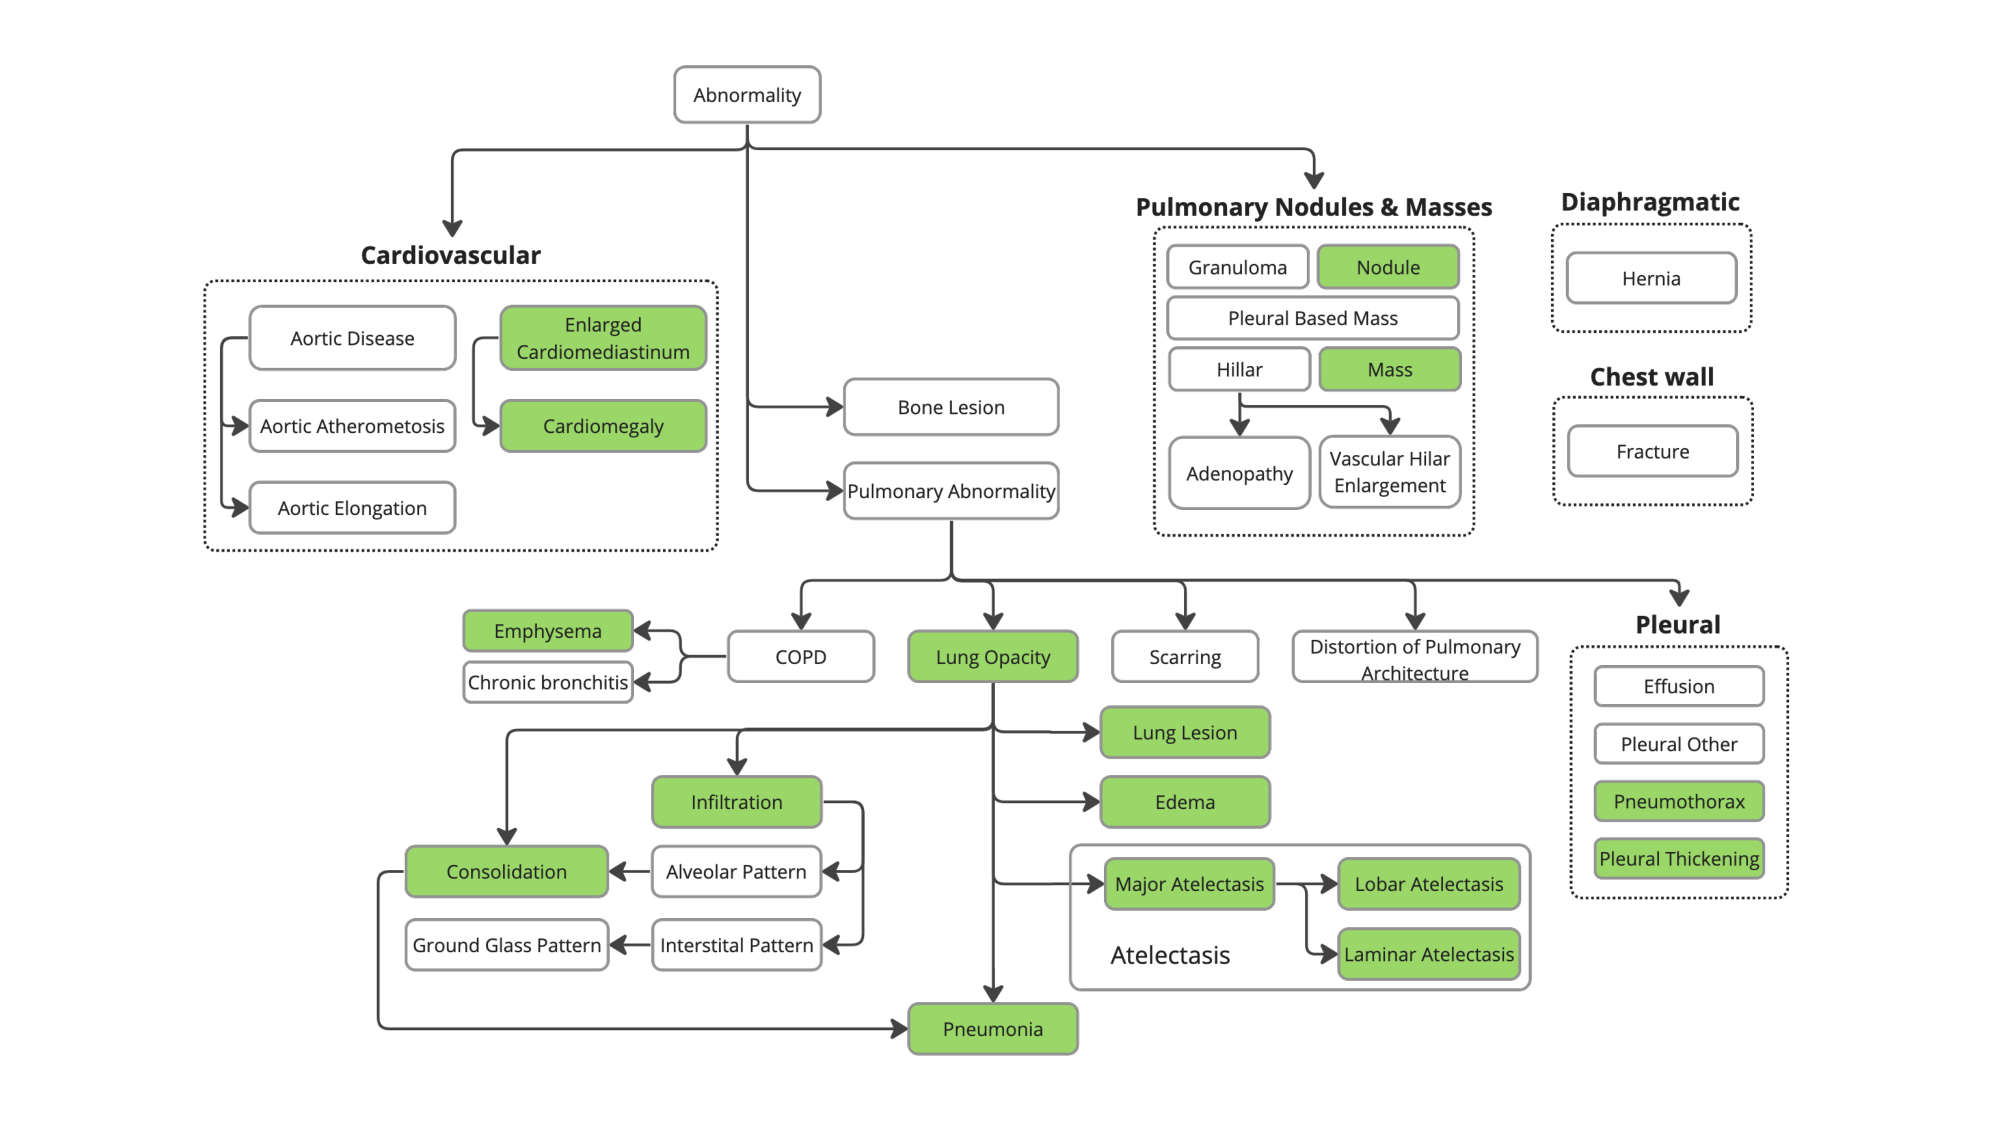
\includegraphics[width=\textwidth]{\figurepath{taxonomy_structure/taxonomy_structure.pdf}}
    \caption{Taxonomy structure of lung pathologies in chest radiographs.}%
    \label{fig:taxonomy.fig.1.taxonomy_structure}
\end{figure}
In this study, we investigated the frequency of various pathological labels in three distinct medical imaging datasets: CheX~\cite{irvin_CheXpert_2019}, PADCHEST~\cite{bustos_Padchest_2020}, NIH~\cite{wang_ChestXRay8_2017}. Table~\ref{tab:taxonomy.table.1.datasets.pathologies} depicts the presence of each pathology label across these datasets. To conform to cohen~\cite{cohen_TorchXRayVision_2022} work, the same 18 pathologies selected by Cohen~\cite{cohen_TorchXRayVision_2022} are used for model optimization. Special consideration is given to the pathologies that appear in at least two of the three datasets and are included in our taxonomy. These pathologies are marked with a \colorbox{mygreen}{green} color in the table and include \textbf{Atelectasis}, \textbf{Consolidation}, \textbf{Infiltration}, \textbf{Edema}, \textbf{Pneumonia}, \textbf{Cardiomegaly}, \textbf{Lung Lesion}, \textbf{Lung Opacity}, \textbf{Enlarged Cardiomediastinum}. This selection is significant because it reflects the pathologies that not only manifest more frequently across multiple data sources, but are also reflected in the hierarchical taxonomy used in our study. The study's analysis and conclusions are focused on these specific pathologies due to their consistent presence and relevance within the taxonomy structure. Further, the cross-dataset presence of these pathologies enhances the generalizability of our study, as the developed models are validated on multiple independent datasets. The pathologies that are not highlighted, i.e., those occurring in just one or none of the datasets or not included in our taxonomy, were not included in the final evaluation of this study. Their exclusion is mainly due to the lack of sufficient data for a robust comparison or their non-alignment with the studied taxonomy structure.
\begin{table}[htbp]
\centering
\caption{Pathologies present in each dataset}%
\label{tab:taxonomy.table.1.datasets.pathologies}
\resizebox{\textwidth}{!}{\begin{tabular}{lcccrlccc}
\cellcolor[HTML]{79A8A4}{\color[HTML]{FFFFFF} \textbf{Pathologies}} & \cellcolor[HTML]{79A8A4}{\color[HTML]{FFFFFF} \textbf{NIH}} & \cellcolor[HTML]{79A8A4}{\color[HTML]{FFFFFF} \textbf{PADCHEST}} & \cellcolor[HTML]{79A8A4}{\color[HTML]{FFFFFF} \textbf{CheX}} & \textbf{} & \cellcolor[HTML]{79A8A4}{\color[HTML]{FFFFFF} \textbf{Pathologies}} & \cellcolor[HTML]{79A8A4}{\color[HTML]{FFFFFF} \textbf{NIH}} & \cellcolor[HTML]{79A8A4}{\color[HTML]{FFFFFF} \textbf{PADCHEST}} & \cellcolor[HTML]{79A8A4}{\color[HTML]{FFFFFF} \textbf{CheX}} \\
{Air Trapping} &  & X &  &  & {Hemidiaphragm Elevation} &  & X &  \\
{Aortic   Atheromatosis} &  & X &  &  & \textbf{Hernia} & X & X &  \\
{Aortic Elongation} &  & X &  &  & {Hilar Enlargement} &  & X &  \\
{Aortic   Enlargement} &  &  &  &  & {ILD} &  &  &  \\
\cellcolor[HTML]{E9ECE6}\textbf{Atelectasis} & \cellcolor[HTML]{E9ECE6}X & \cellcolor[HTML]{E9ECE6}X & \cellcolor[HTML]{E9ECE6}X &  & \cellcolor[HTML]{E9ECE6}\textbf{Infiltration} & \cellcolor[HTML]{E9ECE6}X & \cellcolor[HTML]{E9ECE6}X & \cellcolor[HTML]{E9ECE6} \\
{Bronchiectasis} &  & X &  &  & \cellcolor[HTML]{E9ECE6}\textbf{Lung Lesion} & \cellcolor[HTML]{E9ECE6} & \cellcolor[HTML]{E9ECE6} & \cellcolor[HTML]{E9ECE6}X \\
{Calcification} &  &  &  &  & \cellcolor[HTML]{E9ECE6}\textbf{Lung Opacity} & \cellcolor[HTML]{E9ECE6} & \cellcolor[HTML]{E9ECE6} & \cellcolor[HTML]{E9ECE6}X \\
{Calcified   Granuloma} &  &  &  &  & \textbf{Mass} & X & X & \\
\cellcolor[HTML]{E9ECE6}\textbf{Cardiomegaly} & \cellcolor[HTML]{E9ECE6}X & \cellcolor[HTML]{E9ECE6}X & \cellcolor[HTML]{E9ECE6}X &  & {Nodule/Mass} &  &  &  \\
\cellcolor[HTML]{E9ECE6}\textbf{Consolidation} & \cellcolor[HTML]{E9ECE6} & \cellcolor[HTML]{E9ECE6}X & \cellcolor[HTML]{E9ECE6}X &  & \textbf{Nodule} & X & X & \\
{Costophrenic   Angle Blunting} &  & X &  & \multicolumn{1}{l}{} & \textbf{Pleural Other} &  &  & X \\
\cellcolor[HTML]{E9ECE6}\textbf{Edema} & \cellcolor[HTML]{E9ECE6}X & \cellcolor[HTML]{E9ECE6}X & \cellcolor[HTML]{E9ECE6}X &  & \textbf{Pleural Thickening} & X & X &  \\
\textbf{Effusion} & X & X & X &  & \cellcolor[HTML]{E9ECE6}\textbf{Pneumonia} & \cellcolor[HTML]{E9ECE6}X & \cellcolor[HTML]{E9ECE6}X & \cellcolor[HTML]{E9ECE6}X \\
\textbf{Emphysema} & X & X &  &  & \textbf{Pneumothorax} & X & X & X \\
\cellcolor[HTML]{E9ECE6}\textbf{Enlarged   Cardiomediastinum} & \cellcolor[HTML]{E9ECE6} & \cellcolor[HTML]{E9ECE6} & \cellcolor[HTML]{E9ECE6}X & \multicolumn{1}{l}{} & {Pulmonary Fibrosis} &  &  &  \\
\textbf{Fibrosis} & X & X &  &  & {Scoliosis} &  & X &  \\
{Flattened   Diaphragm} &  & X &  &  & {Tuberculosis} &  & X &  \\
{Fracture} &  & X & X &  & {Tube} &  & X &  \\
{Granuloma} &  & X &  &  &  & \multicolumn{1}{l}{} & \multicolumn{1}{l}{} & \multicolumn{1}{l}{}
\end{tabular}}
\end{table}
Table~\ref{tab:taxonomy.table.2.datasets.ninstances} shows the number of instances that has a specific pathology in each of the three studied datasets (CheX~\cite{irvin_CheXpert_2019}, PADCHEST~\cite{bustos_Padchest_2020}, NIH~\cite{wang_ChestXRay8_2017}). Prior to applying the proposed technique a set of preprocessing steps are applied to ground truth label set. In medical images with multiple classes, it is common for the labeler to only label the pathologies that their study requires. This sometimes result in situations where some instances of data are labeled for the presence of some of the child pathologies but not their corresponding parent pathologies. To compensate for this lack of labeling for some parent classes which is necessary for the effectiveness of the proposed techniques, we updated the label value indicating the presence of classes with at least one child class to \textcolor{blue}{TRUE} (indicating the class exist in that instance). This preprocessing is applied to all pathologies which are not labeled in the original ground truth label set. As can be seen in Table~\ref{tab:taxonomy.table.2.datasets.ninstances} (\colorbox{mygreen}{highlighted cells}), while the Lung Opacity and Enlarged Cardiomediastinum classes were not present in the original ground truth label sets of NIH and PADCHEST datasets (Table~\ref{tab:taxonomy.table.1.datasets.pathologies}), by updating the ground truth label set we end up with multiple instances where based on the presence of their child classes' presence we have determined the presence of the respective parent class.
\begin{table}[H]
\centering
\caption{Number of samples present in the evaluated datasets (CheX, NIH, and PC) per pathology.}%
\label{tab:taxonomy.table.2.datasets.ninstances}
\begin{tabular}{lcccccc}
\rowcolor[HTML]{79A8A4}
\multicolumn{1}{c}{\cellcolor[HTML]{79A8A4}{\color[HTML]{FFFFFF} }} & \multicolumn{2}{c}{\cellcolor[HTML]{79A8A4}{\color[HTML]{FFFFFF} \textbf{CheXpert}}} & \multicolumn{2}{c}{\cellcolor[HTML]{79A8A4}{\color[HTML]{FFFFFF} \textbf{NIH}}} & \multicolumn{2}{c}{\cellcolor[HTML]{79A8A4}{\color[HTML]{FFFFFF} \textbf{PADCHEST}}} \\
\rowcolor[HTML]{79A8A4}
\multicolumn{1}{c}{\multirow{-2}{*}{\cellcolor[HTML]{79A8A4}{\color[HTML]{FFFFFF} \textbf{Pathologies\textbackslash{}Dataset}}}} & {\color[HTML]{FFFFFF} PA} & {\color[HTML]{FFFFFF} AP} & {\color[HTML]{FFFFFF} PA} & {\color[HTML]{FFFFFF} AP} & {\color[HTML]{FFFFFF} PA} & {\color[HTML]{FFFFFF} AP} \\
\textbf{Atelectasis} & 2460 & 11643 & 1557 & 1016 & 2419 & 232 \\
\textbf{Consolidation} & 1125 & 4956 & 384 & 253 & 475 & 77 \\
\textbf{Infiltration} & 0 & 0 & 3273 & 1131 & 4309 & 587 \\
\textbf{Pneumothorax} & 1060 & 4239 & 243 & 253 & 97 & 15 \\
\textbf{Edema} & 1330 & 15117 & 39 & 237 & 108 & 130 \\
\textbf{Emphysema} & 0 & 0 & 264 & 193 & 546 & 30 \\
\textbf{Fibrosis} & 0 & 0 & 556 & 61 & 341 & 8 \\
\textbf{Effusion} & 5206 & 19349 & 1269 & 654 & 1625 & 311 \\
\textbf{Pneumonia} & 992 & 2064 & 175 & 89 & 1910 & 211 \\
\textbf{Pleural\_Thickening} & 0 & 0 & 745 & 145 & 2075 & 34 \\
\textbf{Cardiomegaly} & 2117 & 8284 & 729 & 203 & 5387 & 261 \\
\textbf{Nodule} & 0 & 0 & 1609 & 460 & 2190 & 95 \\
\textbf{Mass} & 0 & 0 & 1213 & 493 & 506 & 17 \\
\textbf{Hernia} & 0 & 0 & 81 & 13 & 988 & 38 \\
\textbf{Lung Lesion} & 1655 & 3110 & 0 & 0 & 0 & 0 \\
\textbf{Fracture} & 1115 & 3463 & 0 & 0 & 1662 & 69 \\
\textbf{Lung Opacity} & 7006 & 28183 & \cellcolor[HTML]{E9ECE6}4917 & \cellcolor[HTML]{E9ECE6}2216 & \cellcolor[HTML]{E9ECE6}6947 & \cellcolor[HTML]{E9ECE6}861 \\
\textbf{Enlarged Cardiomediastinum} & 1100 & 4577 & \cellcolor[HTML]{E9ECE6}729 & \cellcolor[HTML]{E9ECE6}203 & \cellcolor[HTML]{E9ECE6}5387 & \cellcolor[HTML]{E9ECE6}261 \\
\rowcolor[HTML]{79A8A4}
{\color[HTML]{FFFFFF} Total} & {\color[HTML]{FFFFFF} 20543} & {\color[HTML]{FFFFFF} 53359} & {\color[HTML]{FFFFFF} 28868} & {\color[HTML]{FFFFFF} 9060} & {\color[HTML]{FFFFFF} 61692} & {\color[HTML]{FFFFFF} 2445}
\end{tabular}
\end{table}
Figure~\ref{fig:taxonomy.fig.3.roc_curve_all_datasets} presents the comparison of the performance of our proposed techniques ``logit'' and ``loss'' against the ``baseline'' technique for a series of nine medical conditions related to lung and heart diseases on three datasets (CheXpert, PADCHEST, NIH). These nine pathologies include the two parent classes (\textbf{Lung Opacity}, and \textbf{Enlarged Cardiomediastinum}) and their corresponding child classes, as shown in Figure~\ref{fig:taxonomy.fig.1.taxonomy_structure}. The individual subplots exhibit overlaid receiver operating characteristic (ROC) curves and their corresponding AUC scores.
\begin{figure}[H]
    \centering
    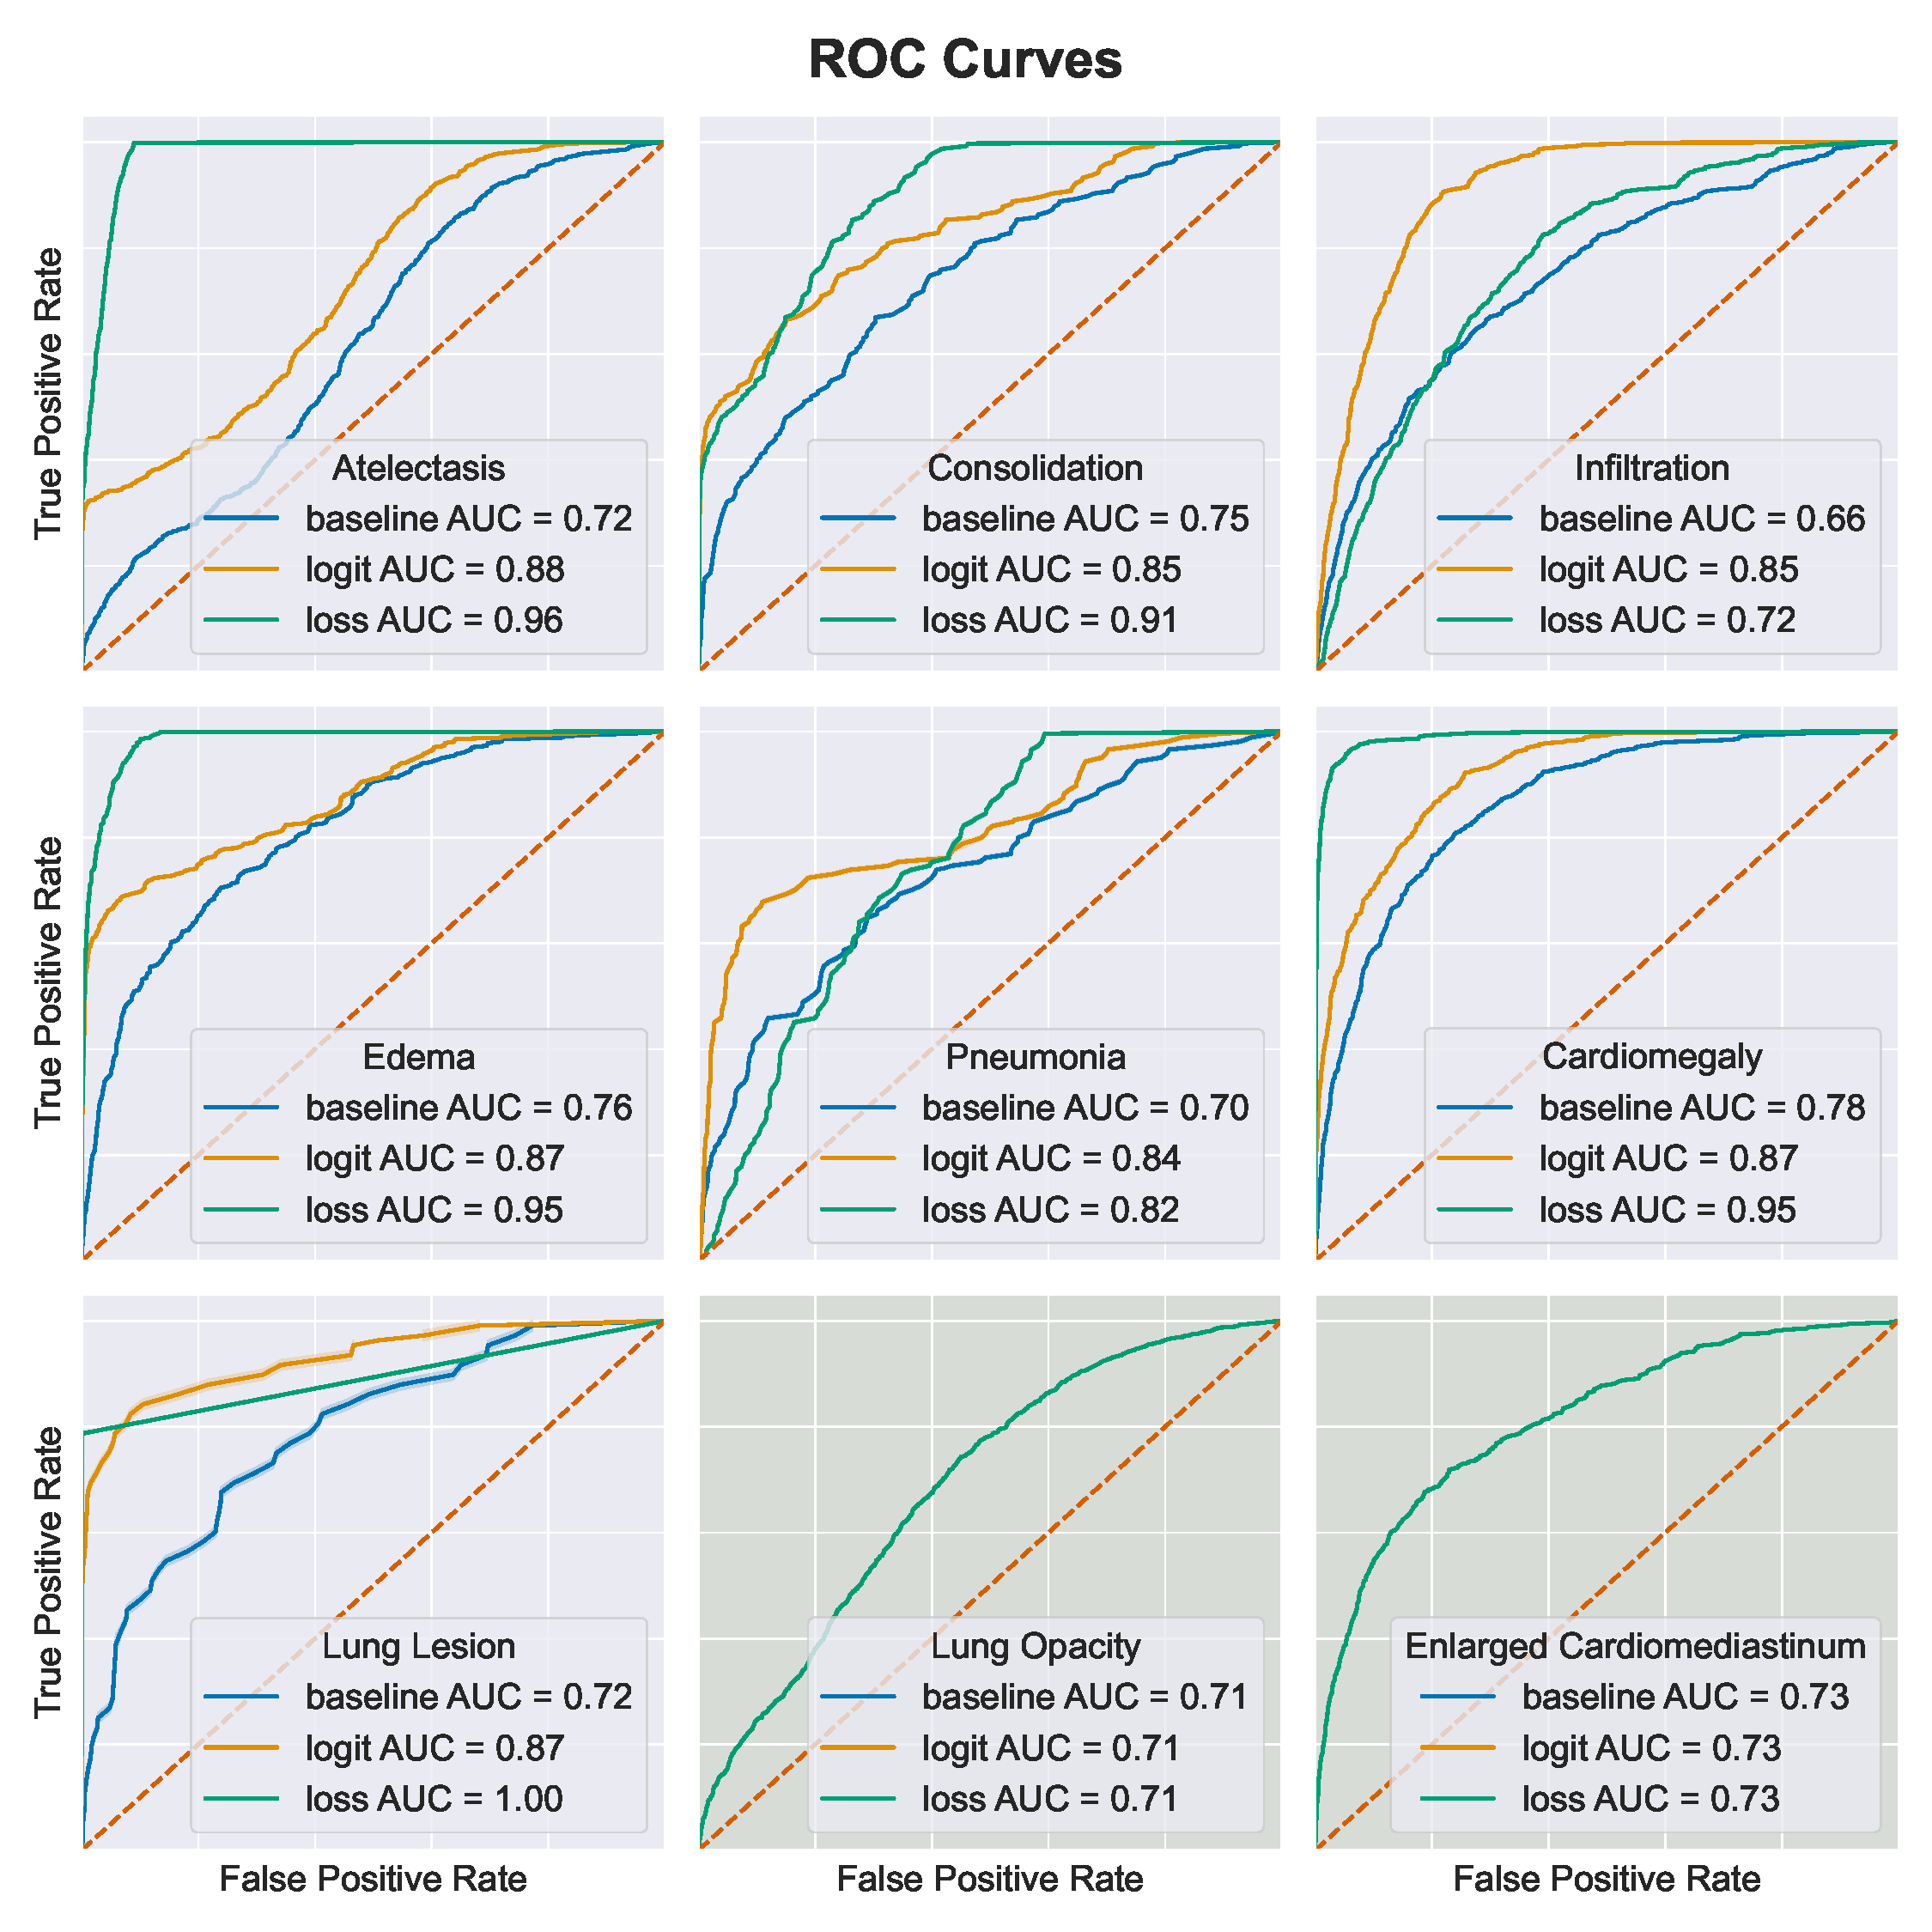
\includegraphics[width=\textwidth]{\figurepath{roc_curve_all_datasets/ROC/roc_curve_all_datasets.pdf}}
    \caption{Comparative analysis of the ROC curves for nine thoracic pathologies using the ``logit'' and ``loss'' techniques as well as the baseline. The subplots highlighted with a darker background, represent parent class diseases.}%
    \label{fig:taxonomy.fig.3.roc_curve_all_datasets}%
\end{figure}
Table~\ref{tab:taxonomy.table.3.metrics} presents the comparison of the performance of our proposed techniques ``logit'' and ``loss'' against the ``baseline'' technique for various statistical metrics. The ``logit'' method (upper table), shows a considerable improvement over the ``baseline'' across all conditions. We observe kappa values between 0.495 and 1. The kappa statistic is a measure of agreement between two methods, with a value of 1 indicating perfect agreement. The p-value for all child classes show a value less than 0.05 (ranging from 2.1E-89 to 2.9E-16), which indicates the statistically significant superiority of the ``logit'' method over the ``Baseline''. High t-statistics and power values of 1 further confirm the robustness of our method. In terms of Bayes factor, results for the ``logit'' method are extremely strong for all conditions suggesting a high amount of evidence in favor of the ``logit'' method for these conditions. The second proposed method, ``loss'', also presents promising results when compared to the ``baseline'', but with more variation. Kappa values ranged from a low of 0.059 for Lung Lesion to a high of 0.836 for Infiltration. The p-values indicate statistically significant differences for most conditions, although Infiltration and Pneumonia present p-values greater than 0.05 (0.053 and 0.207 respectively), suggesting that the performance improvement over the ``baseline'' for these conditions may not be statistically significant. T-statistics are high, and power values are 1 for all conditions except Infiltration and Pneumonia. The cohen-d values for this method are generally larger than those in the ``logit'' method, indicating a larger effect size. In terms of Bayes factor, results for the ``loss'' method are extremely strong for conditions such as Atelectasis and Edema, while being much lower for conditions like Infiltration and Pneumonia, suggesting a reduced amount of evidence in favor of the ``loss'' method for these conditions. Both the ``logit'' and ``loss'' methods show significant improvements over the ``baseline'' method in the diagnosis of several heart and lung conditions, albeit with some variance in the degree of improvement. While the ``logit'' method demonstrates a more consistent level of improvement across all conditions, the ``loss'' method shows potential for even greater improvement in certain conditions but with less consistency across the conditions studied.
\begin{table}[H]
\centering
\caption{Statistical performance comparison between the proposed techniques ``logit'' and ``loss'' and the ``baseline'' technique across various pathologies. The upper table displays the findings of the ``logit'' technique, while the lower table displays the findings of the ``loss'' technique. The reported metrics for each pathology are the Kappa statistic, p-value, t-statistic, statistical power, Cohen's d, and Bayes Factor (BF10). A kappa value of 1 indicates perfect agreement between techniques, whereas a larger Bayes factor indicates greater support for the ``logit'' or ``loss'' technique over the baseline.}%
\label{tab:taxonomy.table.3.metrics}
\resizebox{\textwidth}{!}{%
%! suppress = EscapeAmpersand
\begin{tabular}{clrrrrrr}
 & \cellcolor[HTML]{79A8A4}{\color[HTML]{FFFFFF} } & \cellcolor[HTML]{79A8A4}{\color[HTML]{FFFFFF} kappa} & \cellcolor[HTML]{79A8A4}{\color[HTML]{FFFFFF} p\_value} & \cellcolor[HTML]{79A8A4}{\color[HTML]{FFFFFF} t\_stat} & \cellcolor[HTML]{79A8A4}{\color[HTML]{FFFFFF} power} & \cellcolor[HTML]{79A8A4}{\color[HTML]{FFFFFF} cohen-d} & \cellcolor[HTML]{79A8A4}{\color[HTML]{FFFFFF} BF10} \\
 & Atelectasis & 0.495 & 2.1E-89 & 20.2 & 1 & 0.346 & 3.0E+85 \\
 & Consolidation & 0.508 & 2.0E-18 & 8.8 & 1 & 0.150 & 8.3E+14 \\
 & Infiltration & 0.620 & 2.7E-28 & 11.1 & 1 & 0.190 & 4.9E+24 \\
 & Edema & 0.614 & 1.2E-52 & 15.3 & 1 & 0.263 & 7.2E+48 \\
 & Pneumonia & 0.573 & 2.9E-16 & 8.2 & 1 & 0.140 & 6.3E+12 \\
 & Cardiomegaly & 0.615 & 1.9E-72 & 18.1 & 1 & 0.310 & 3.9E+68 \\
 & Lung Lesion & 0.580 & 7.0E-23 & 9.9 & 1 & 0.169 & 2.1E+19 \\
 & Lung Opacity & 1 & 1 & 0 & 0.05 & 0 & 0.019 \\
\multirow{-10}{*}{\begin{tabular}[c]{@{}c@{}}\\ L\\  \\ O\\ \\ G\\ \\ I\\ \\ T\end{tabular}} & Enlarged Cardiomediastinum & 1 & 1 & 0 & 0.05 & 0 & 0.019 \\
\multicolumn{8}{l}{{\color[HTML]{FFFFFF} }} \\
 & \cellcolor[HTML]{79A8A4}{\color[HTML]{FFFFFF} } & \cellcolor[HTML]{79A8A4}{\color[HTML]{FFFFFF} kappa} & \cellcolor[HTML]{79A8A4}{\color[HTML]{FFFFFF} p\_value} & \cellcolor[HTML]{79A8A4}{\color[HTML]{FFFFFF} t\_stat} & \cellcolor[HTML]{79A8A4}{\color[HTML]{FFFFFF} power} & \cellcolor[HTML]{79A8A4}{\color[HTML]{FFFFFF} cohen-d} & \cellcolor[HTML]{79A8A4}{\color[HTML]{FFFFFF} BF10} \\
 & Atelectasis & 0.222 & 4.9E-183 & 29.3 & 1 & 0.502 & 7.7E+178 \\
 & Consolidation & 0.310 & 4.3E-116 & 23.1 & 1 & 0.396 & 1.2E+112 \\
 & Infiltration & 0.836 & \multicolumn{1}{l}{0.053} & 1.9 & 0.49 & 0.033 & 0.125 \\
 & Edema & 0.343 & 4.4E-190 & 29.9 & 1 & 0.512 & 8.2E+185 \\
 & Pneumonia & 0.394 & \multicolumn{1}{l}{0.207} & 1.3 & 0.24 & 0.022 & 0.043 \\
 & Cardiomegaly & 0.501 & 1.2E-101 & 21.6 & 1 & 0.370 & 4.7E+97 \\
 & Lung Lesion & 0.059 & 1.2E-207 & 31.3 & 1 & 0.537 & 2.9E+203 \\
 & Lung Opacity & 1 & 1 & 0 & 0.05 & 0 & 0.019 \\
\multirow{-10}{*}{\begin{tabular}[c]{@{}c@{}}\\ L\\ \\ O\\ \\ S\\ \\ S\end{tabular}} & Enlarged Cardiomediastinum & 1 & 1 & 0 & 0.05 & 0 & 0.019
\end{tabular}%
}
\end{table}
Figure~\ref{fig:taxonomy.fig.2.metrics} compares the performance of the proposed ``loss'' and ``logit'' techniques to the ``baseline'' across three key metrics: accuracy (ACC), area under the receiver operating characteristic curve (AUC), and F1 score for various pathologies.
The accuracy metric presents a clear advantage for the ``loss'' and ``logit'' methods over the ``baseline'' for the child classes of pathologies, a pattern that is consistent with the kappa statistics presented earlier. For example, in Atelectasis, the ``loss'' method has an accuracy of 0.922 compared to 0.686 for the ``baseline'', while the ``logit'' method stands at 0.874. As expected, the parent classes, lung opacity and enlarged cardiomediastinum, show no difference between the techniques, with an accuracy of 0.663 and 0.696, respectively.
The AUC, a model performance metric that accounts for both sensitivity and specificity, demonstrates once more that the ``loss'' and ``logit'' methods for the child classes are superior. For example, in the case of cardiomegaly, the AUC is improved by 21\% and 11\% using the loss and logit methods, respectively. The AUC values for lung opacity and an enlarged cardiomediastinum, the parent classes, are identical for all three methods.
The F1 score, which is the harmonic mean of precision and recall, sheds additional light on the enhanced performance of our proposed techniques. Notably, lung lesion increases from 0.094 in the ``baseline'' method to 0.982 in the ``loss'' method and 0.263 in the ``logit'' method.
These results further validate our earlier findings that the ``logit'' and ``loss'' methods provide significant performance improvements over the ``baseline'' method for the majority of the child classes. Across all metrics and conditions, the ``loss'' method appears to perform marginally better than the ``logit'' method.
\begin{figure}[H]
    \centering
    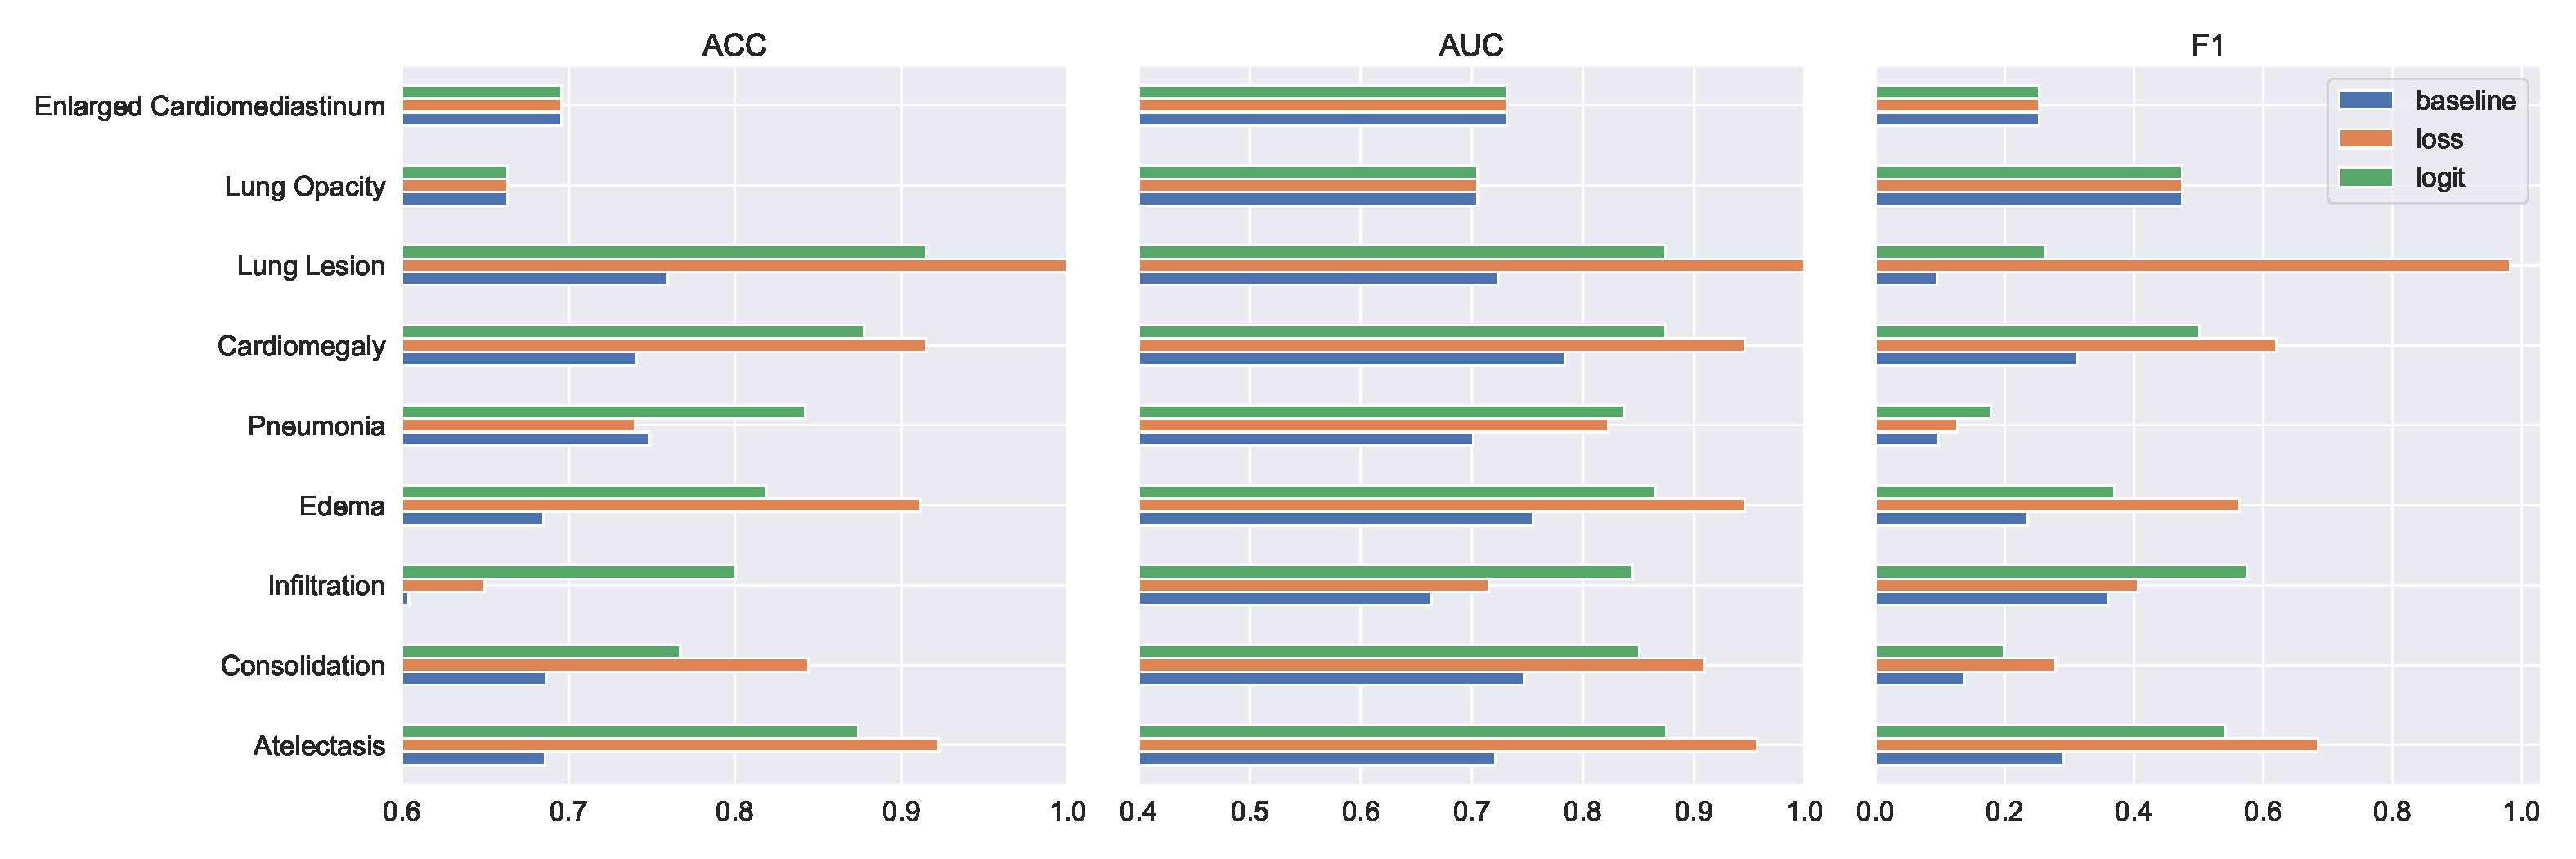
\includegraphics[width=\textwidth]{\figurepath{auc_acc_f1_all_datasets/ROC/metrics_AUC_ACC_F1.pdf}}
    \caption{Heatmap visualization of model performance metrics across all three datasets. The subplots from left to right correspond to the Accuracy (ACC), Area Under the ROC Curve (AUC), and F1 Score for the baseline, ``loss'', and ``logit'' techniques respectively. The pathologies are shared on the y-axis. Darker colors signify higher values, indicating better model performance. Each cell represents the value of the corresponding metric for the given technique on a specific pathology}%
    \label{fig:taxonomy.fig.2.metrics}
\end{figure}
\section{Discussion and Conclusion}\label{sec:taxonomy.discussion}
In this work, we presented two hierarchical multi-label classification methods aimed at enhancing thoracic disease diagnosis in chest radiography. The first approach, denoted as the ``loss'' method, refines the loss value for each pathology, factoring in the influence of parent pathologies in the hierarchical structure.  The ``logit'' method is a powerful tool for improving the performance of pre-trained models. This approach updates the logit values of each pathology based on the corresponding logit values of their parent pathologies, leveraging the inherent taxonomical relationships between pathologies. This strategy is particularly useful when ground truth labels are not readily available, as it allows for efficient enhancement of model performance without requiring access to such labels. By avoiding the need to build new models from scratch, the ``logit'' method offers a streamlined and effective approach to optimizing model performance in a variety of contexts. Whether working with complex medical data or other types of information, this approach can help researchers and practitioners achieve more accurate and reliable results with greater ease and efficiency.
The results of the study demonstrate the effectiveness of proposed hierarchical multi-label classification methodologies in improving the precision of thoracic disease diagnosis. Various performance metrics, including accuracy, AUC, and F1 scores, as well as Cohen's d, Cohen's kappa, t-statistics, p-value, and Bayes factor, are used to evaluate the performance of the proposed techniques against the baseline on three public datasets (CheXpert~\cite{irvin_CheXpert_2019}, PADCHEST~\cite{bustos_Padchest_2020}, and NIH~\cite{wang_ChestXRay8_2017}), showing substantial improvements in the proposed techniques against the baseline. These findings suggest that these methods can be used as reliable tools for accurate and efficient diagnosis of thoracic diseases. Further research is needed to explore the potential benefits of these methods in clinical practice.
The utilization of logit adjustments represents a simple yet powerful approach for incorporating label hierarchy into a model without requiring significant modifications to the existing framework. However, this approach has the potential to obscure the optimization and learning process and results. On the other hand, modifying loss values is more closely aligned with the optimization process of the model, enabling a more refined adjustment of the hierarchical influence through weighting factors. This methodology promotes resilience to inaccuracies in labeling and improves conformity with established hierarchical relationships.
In essence, both the ``loss'' and ``logit'' techniques effectively leverage disease taxonomy to bolster classification performance, reinforcing the significance of exploiting label relationships in classification tasks. Moreover, these hierarchical techniques can potentially aid clinicians by improving the interpretability of the models' predictions. Exploring predictions at varying levels of granularity based on taxonomy could facilitate personalized diagnoses tailored to individual clinical needs.  Additionally, the techniques could be integrated into computer-aided diagnosis systems to provide more accurate and efficient diagnoses, potentially reducing the workload of clinicians and improving patient outcomes.
However, these methodologies exhibit certain constraints. Extending these methodologies to other applications would necessitate the development of a taxonomical structure for the labels of the corresponding dataset. The construction of such a structure may present difficulties for complex applications and typically necessitates the consensus of multiple domain experts. Additionally, the performance of the proposed techniques may be influenced by the quality and consistency of the labeling in the datasets, which may vary across different sources. Future studies should aim to evaluate the techniques on a broader range of datasets and consider the impact of labeling quality on performance.
\section*{Appendices}
\section*{Acknowledgements}
